\documentclass[11pt]{article}
\usepackage{amsmath, amssymb}
\usepackage{geometry}
\geometry{margin=1in}
\usepackage{fancyhdr}
\usepackage{lastpage}
\usepackage{parskip} % Better paragraph spacing
\usepackage{titlesec} % Better section formatting
\usepackage{graphicx}
\usepackage{float}
\usepackage[most]{tcolorbox}
\usepackage{lmodern}
\usepackage{caption}

% Define commands for reusable content
\newcommand{\coursename}{CS-401 Applied Data Analysis}
\newcommand{\lecturenum}{02}
\newcommand{\lecturedate}{\today}

% Configure section spacing
\titlespacing*{\section}{0pt}{2ex plus 1ex minus .2ex}{1.5ex plus .2ex}
% Header / Footer
\pagestyle{fancy}
\fancyhf{}
\fancyhead[L]{\coursename}
\fancyhead[R]{Lecture \lecturenum}
\fancyfoot[L]{EPFL - Computer Science}
\fancyfoot[C]{Author: Jonathan Dutoit}
\fancyfoot[R]{Page \thepage\ of \pageref{LastPage}}

\begin{document}

\begin{center}
  {\large EPFL - Computer Science} \\[0.5em]
  {\Large \textbf{\coursename}} \\[0.5em]
  {\large Lecture \lecturenum\ --- \lecturedate} \\[0.5em]
  {\large Author: Jonathan Dutoit} \\
  {\large Professor: Maria Brbic}
\end{center}

\vspace{2cm}

\begin{center}
  {\LARGE \textbf{Handling Data}
\end{center}

\vspace{1cm}

\section*{Lecture overview}

\begin{enumerate}
	\item Data Models
	\item Data Sources
	\item Data wrangling
\end{enumerate}

\section*{Data model}

"A data model is an abstract model that organizes elements of data and standardizes how they relate to one another and to the properties of real-world entities..." - Wikipedia 

\begin{tcolorbox}[
  colback=gray!15,     % background color
  colframe=black!50,    % border color
  boxrule=1pt,       % border thickness
  arc=3mm,             % rounded corners
  left=4mm, right=4mm, top=2mm, bottom=2mm % padding
]
\textbf{Simple definition} \\

A data model specifies how you think about the world.
\end{tcolorbox}

For instance, hospital reports. A patient comes to a hospital and it's record is saved. You can link all data to relationships between patients and doctors. 

\newpage


\textcolor{red}{Q: "How do you think about the world?"}

\textcolor{red}{A: "See my entity-relationship diagram!"}


% Quick centered image
\begin{figure}[H]
    \centering
    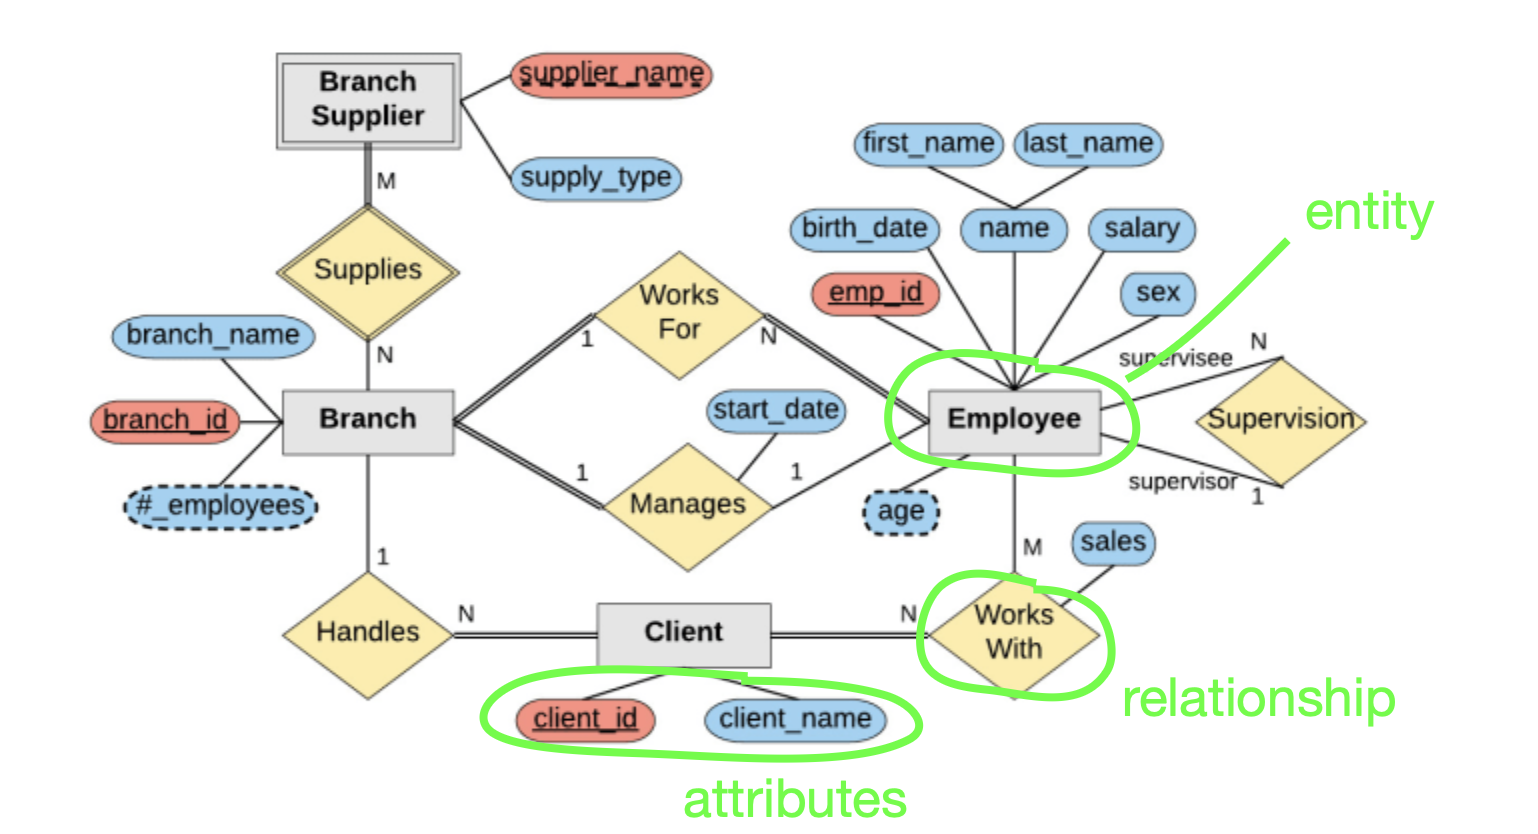
\includegraphics[width=0.85\textwidth]{data-diagram}
    \label{fig:LABEL}
\end{figure}

\begin{tcolorbox}[
  colback=yellow!15,     % background color
  colframe=black!50,    % border color
  boxrule=1pt,       % border thickness
  arc=3mm,             % rounded corners
  left=4mm, right=4mm, top=2mm, bottom=2mm % padding
]
How to store my data on a computer?
\end{tcolorbox}

\textcolor{red}{Q1: "How should I store my data on a computer?"}

\textcolor{red}{Q2: "How do I think about the world?"}


\begin{itemize}
	\item \textbf{Flat model}: The world is simple, one type of entity, all with the same attributes
	\item \textbf{Relational model}: The world contains many types of entities, connected by relationships
	\item \textbf{Document model}: The world is a hierarchy of entities
	\item \textbf{Network model}: The world is a complex network of entities
\end{itemize}

\section*{Flat Model}

\textcolor{blue}{"The world is simple: one type of entity, all with the same attributes"}

\begin{itemize}
	\item Example: log files; e.g., Apache web server (httpd)
	\begin{itemize}
		\item Entities = request from clients to server
	\end{itemize}
	\item Another common format: CSV (“comma-separated vector”)
\end{itemize}

\section*{Relational Model}

\textcolor{blue}{"The world contains many types of entities, connected by relationships"}

\begin{itemize}
	\item The relational model is ubiquitous: 
	\begin{itemize}
		\item MySQL, PostgreSQL, Oracle, DB_2, SQLite, ...
		\item You use it many times every day
	\end{itemize}
	
	\item Data represented as tables describing
	\begin{itemize}
		\item entities
		\item relationship between entities
        \end{itemize}
\end{itemize}

\vspace{1cm}
\textbf{\textcolor{red}{Processing data in the relational model: SQL (Structured Query Language)}}

\begin{itemize}
	\item Declarative language for core data manipulations
	\item You think about what you want, not how to compute it
\end{itemize}

\vspace{0.5cm}
\textbf{\textcolor{red}{SQL}}

\begin{itemize}
	\item You should know basics of SQL
	\item Key operations
	\begin{itemize}
		\item Select (!), update, delete
		\item Unique keys
		\item Joins (inner, left outer, right outer, full)
		\items Sorting
		\item Aggregation (group by, count, min, max, avg, etc.)
	\end{itemize}
\end{itemize}

\vspace{0.5cm} 

\textbf{\textcolor{red}{SQL Implementation}}

% Quick centered image
\begin{figure}[H]
    \centering
    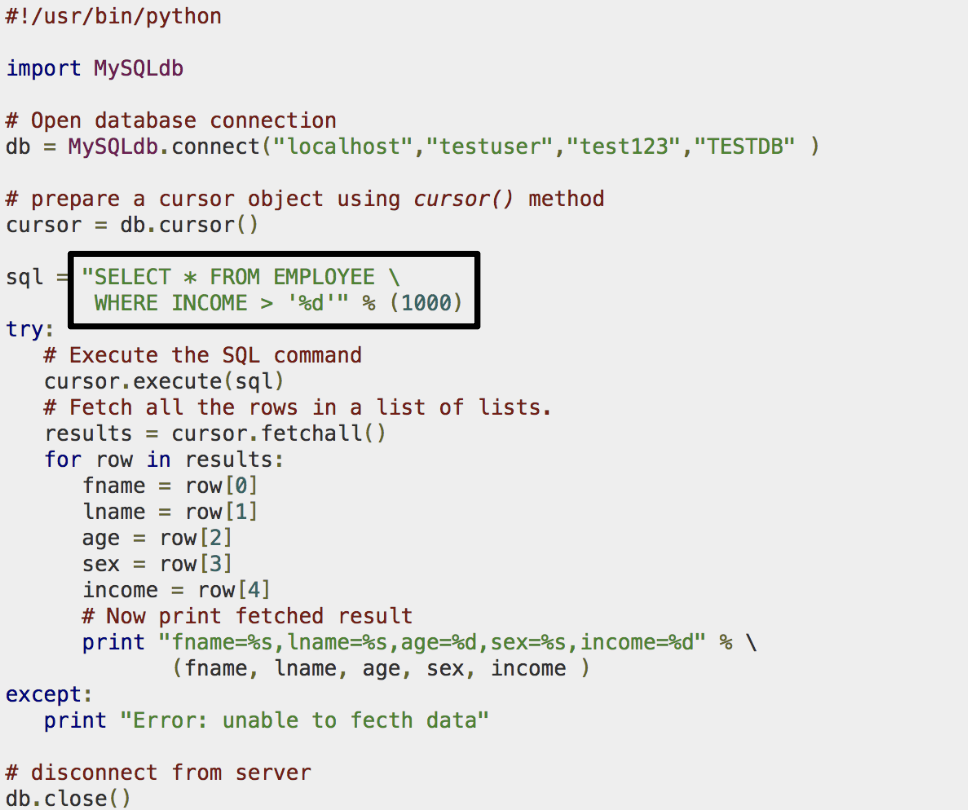
\includegraphics[width=0.7\textwidth]{sql-implementation}
    \label{fig:LABEL}
\end{figure}

\vspace{0.5cm} 

\textbf{\textcolor{red}{"SQL": Pandas (Python Library)}}

\begin{itemize}
	\item Similar to SQL (declarative), with additional elements of functional programming (map(), filter(), etc.)
	\item SQL "table" $\Leftrightarrow$ Pandas "DataFrame"
\end{itemize}


\vspace{0.5cm} 

\textbf{\textcolor{red}{Pandas vs. SQL}}

\textcolor{blue}{+ Pandas is lightweight and fast}

\textcolor{blue}{+ Natively Python, i.e., full SQL expressiveness plus the expressiveness of Python, especially for function evaluation}

\textcolor{blue}{+ Integration with plotting functions like Matplotlib}

\textcolor{red}{- In Pandas, tables must fit into memory}

\textcolor{red}{- No post-load indexing functionality: indices are built when a table is created}

\textcolor{red}{- No transactions, journaling, etc. (matters for parallel applications)}

\textcolor{red}{- Large, complex joins are slower}

\section*{Document Model}

\textcolor{blue}{"The world is a hierarchy of entities"}

\begin{itemize}
	\item XML format
	\item JSON format
\end{itemize}

\vspace{0.5cm}

\begin{tcolorbox}[
  colback=gray!15,     % background color
  colframe=black!50,    % border color
  boxrule=1pt,       % border thickness
  arc=3mm,             % rounded corners
  left=4mm, right=4mm, top=2mm, bottom=2mm % padding
]

\textbf{\textcolor{red}{Think for a minute:}} \\

\textbf{If we want to use relational DB (e.g., MySQL) instead of XML, how can we store several phone numbers for the same person?} \\

\textbf{Answer:} Separate it in two tables. For instance, a new table of phone numbers. Here, the \textbf{Document Model} is more suitable than the \textbf{Relational Model} because everything is done in the same place, you just need to change one entry. 
\end{tcolorbox}

\vspace{0.5cm}


\textbf{\textcolor{red}{Processing XML and JSON}}

\begin{itemize}
	\item Document structure = tree
	\item Processing via tree traversal (depth- or breadth-first search)
	\item Or use proper query language, such as XQuery or jg
\end{itemize}

\newpage


\section*{Network Model}

\textcolor{blue}{"The world is a complex network of entities"}

% Quick centered image
\begin{figure}[H]
    \centering
    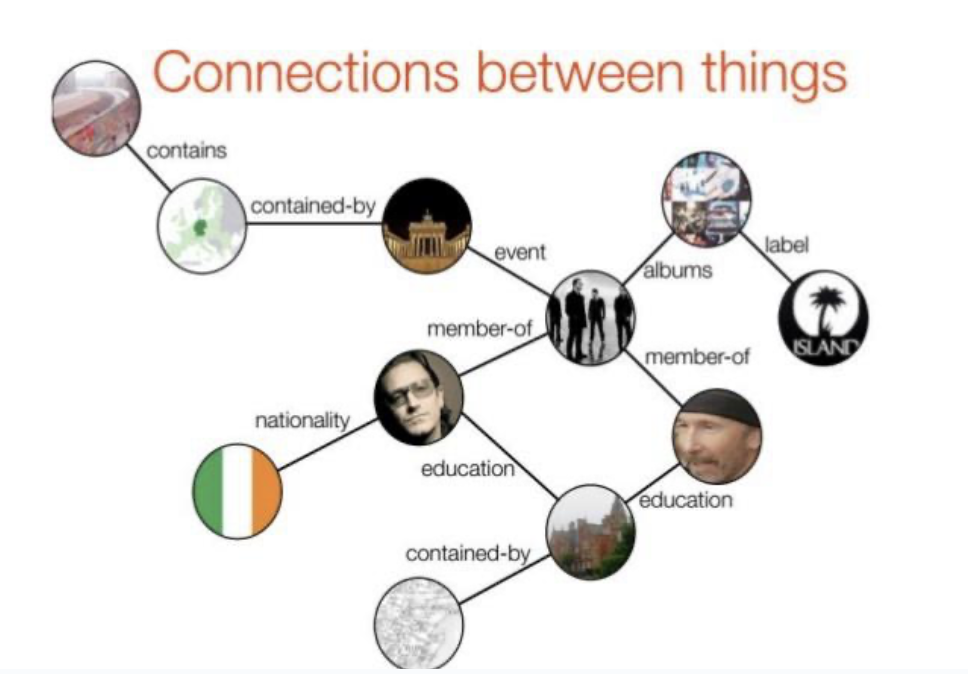
\includegraphics[width=0.5\textwidth]{network-graph}
    \label{fig:LABEL}
\end{figure}

\textbf{\textcolor{red}{"How should I store my data on a computer?"}}

\textbf{\textcolor{red}{-- A word (or two) on binary format}}

\begin{itemize}
	\item "Parsing" = converting strings (as stored in text files) to data types used by computer programs (e.g., int, float, boolean, array, list)
	\item Possibly expensive, but can be avoided by using binary formats: store data to disk "as is", without first converting to strings
	\item Modern binary formats support nested structures, various levels of schema enforcement, compression, etc.
	\item Python pickle, Java Serializable, Protocol Buffers (Google), ...
\end{itemize}

\textcolor{red}{$\Rightarrow$ Consider converting to a binary format at the beginning of your processing pipeline (especially when using "big data"}

\newpage

\section*{Data Sources}

\textbf{\textcolor{red}{Data sources at Web companies}}

% Quick centered image
\begin{figure}[H]
    \centering
    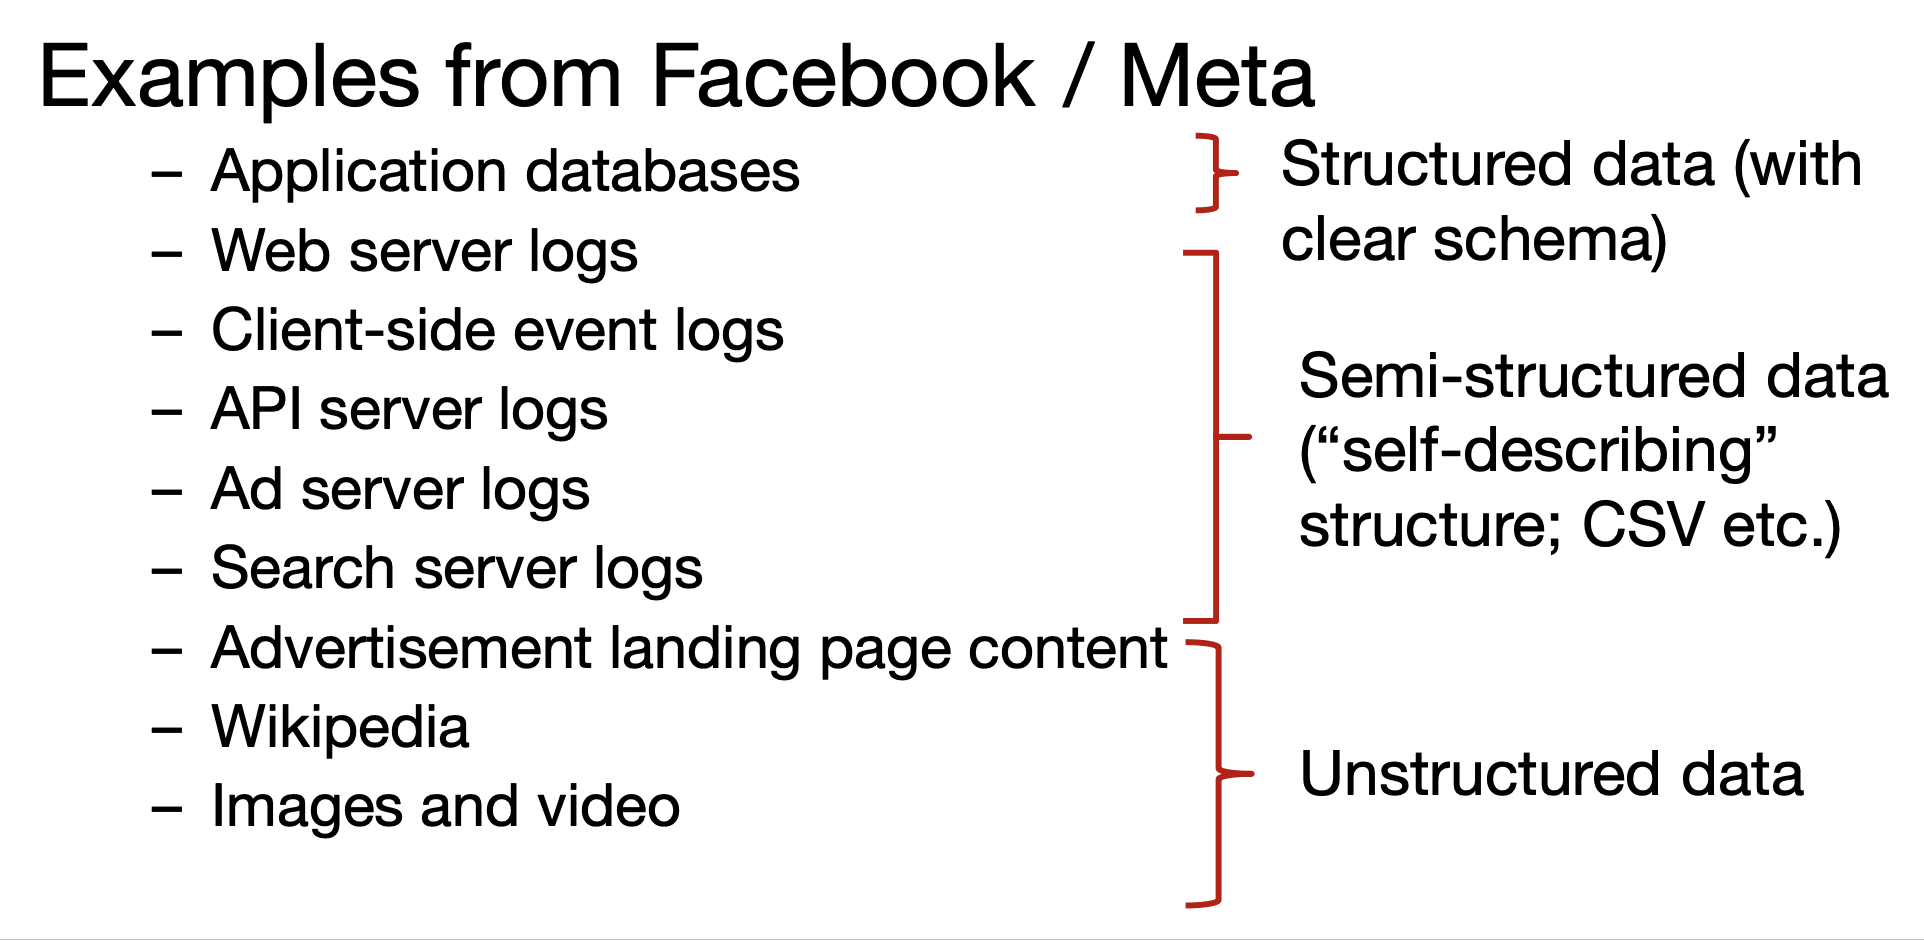
\includegraphics[width=0.7\textwidth]{data-sources}
    \label{fig:LABEL}
\end{figure}
\vspace{0.5cm}

\textbf{\textcolor{red}{Wikipedia}}

\begin{itemize}
	\item 300+ languages
	\item 42 million entities
	\item Mind-boggling richness of data
\end{itemize}

\vspace{0.5cm}

How to work with Wikipedia? 
\begin{itemize}
	\item REST API
	\item XML dumps with wiki markup, SQL database dumps
	\item Issues: Unicode, size, recency, etc.
\end{itemize}

\vspace{0.5cm}

\textbf{\textcolor{red}{Wikidata}}

\begin{itemize}
	\item "Database version" of Wikipedia
	\item \{fr: Suisse, de:Schweiz, it:Svizzera, en:Switzerland, ...\} $\Rightarrow Q39$
	\item Both API access and full database dumps
	\item Available as
	\begin{itemize}
		\item JSON (document model)
		\item RDF (network model)
	\end{itemize}
\end{itemize}

\vspace{0.5cm}

\textbf{\textcolor{red}{Web service}}

\begin{itemize}
	\item Most large web sites today actively discourage "screen-scraping" to get their content
	\item Instead: Web service APIs, for interoperable machine-to-machine interaction over a network
	\item The preferred way to get data from online sources
	\item Most common framework: REST
	\begin{itemize}
		\item You request a URL from the server via HTTP
		\item The server responds with a text file (e.g., JSON, XML, plaintext)
	\end{itemize}
\end{itemize}

\vspace{1cm}

\section*{Data wrangling}

\textbf{\textcolor{red}{Working with raw data sucks}}

\begin{itemize}
	\item Data comes in all shapes and sizes
	\begin{itemize}
		\item CSV files, PDFs, SQL dumps, .jpg, ...
	\end{itemize}
\end{itemize}

\begin{itemize}
        ○ Different files have different formatting
        \begin{itemize}
		\item Empty string or space instead of NULL, extra header rows, character encoding...
        \end{itemize}
\end{itemize}

\begin{itemize}
        ○ "Dirty" data
        \begin{itemize}
		\item Unwanted anomalies, duplicates
        \end{itemize}
\end{itemize}

\vspace{0.5cm}

\textbf{\textcolor{red}{What is data wrangling?}}

\begin{itemize}
	\item \textbf{\textcolor{blue}{Goal:}} extract and standardize the raw data
	\begin{itemize}
		\item Combine multiple data sources
		\item Clean data anomalies
	\end{itemize}
	\item \textbf{\textcolor{green}{Strategy:}} Combine automation with interactive visualizations to aid in cleaning
\end{itemize}

Wrangling takes \textbf{between 50\% and 80\% of your time...}

\vspace{0.5cm}

\textbf{\textcolor{red}{Types of data problems}}

\begin{itemize}
	\item Missing data
	\item Incorrect data
	\item Inconsistent representation of the same data
	\item About 75\% of data problems require human intervention (e.g., experts, crowdsourcing, etc.)
	\item Tradeoff between cleaning data vs, over-sanitizing data
\end{itemize}

\vspace{0.5cm}

\textbf{\textcolor{red}{Diagnosing data problems}}

\begin{itemize}
	\item Visualization and basic stats can convey issues in "raw"data
	\item Different representations highlight different types of issues:
	\begin{itemize}
		\item Outliers often stand out in the right kind of plot
		\item Missing data will cause gaps or zero values in the right kind of plot
	\end{itemize}
	
	\item Becomes increasingly difficult as data gets larger
	\begin{itemize}
		\item Sampling to the rescue!
	\end{itemize}
\end{itemize}


\vspace{0.5cm}

\textbf{\textcolor{red}{Before you start analysing your data}}

\begin{itemize}
	\item "Do I have \textbf{missing data}?" "If data were missing, how could I know?"
	\item "Do I have \textbf{corrupted data?"} (May arise from measurement errors, processing bugs, etc.) 
	\item \textbf{Parse/transform data} into appropriate format for your specific analysis 
	\item Don't be surprised if you need to come back to this stage!
\end{itemize}

\vspace{0.5cm}

\textbf{\textcolor{red}{Desiderata}}

It's always ideal if you can put your hands on the \textbf{code/documentation about the dataset} you are analysing (provenance)

It's always ideal if the provided \textbf{data format is nicely parseable} (otherwise you need regexes, or maybe even pay humans)

\vspace{0.5cm}

\textbf{\textcolor{red}{Highly non-parseable data}}

Entire NY Times archive (since 1851) digitized as of 2015. 

$\Rightarrow$ CAPTCHA to prevent spamming and also to parse data from the archives from humans. 
\end{document}
